\documentclass[10pt,anonymous,review]{acmart}

\title{Extending Programming with Diagrammatic Programming Languages}
\author{Zac Nowicki}
\affiliation{
  \institution{Kagi Inc.}
  \city{Palo Alto}
  \state{CA}
  \country{USA}
}
\email{znowicki@kagi.com}

\author{Paul Tarvydas}
\affiliation{
  \institution{Retired}
  \city{Toronto}
  \state{Ontario}
  \country{Canada}
}
\email{paultarvydas@gmail.com}

\begin{document}

\begin{abstract}

We assert that DPLs - Diagrammatic Programming Languages - can be used as an adjunct syntax for creating programs.

We give an example of a simple DPL syntax and describe a method for creating executable code using diagrams drawn with off-the-shelf graphic editors.
  
Certain forms of expression are more easily expressed in DPL form rather than TPL - textual programming language - form. TPL-only expression of programs can lead to perceived complexity and other problems. The use of DPLs makes it possible to address these sorts of issues using fresh notations.
\end{abstract}

\maketitle

\section{Compilation and Execution}
Compilation and execution of this DPL consists of the steps listed below. Note that the diagrams are rough sketches intentionally simplified
for overview purposes only.

\begin{itemize}

\item filler
  
\item Convert DPL program diagrams to JSON.

  \begin{figure}[h]
    \centering
    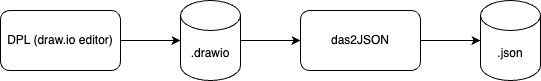
\includegraphics[width=0.8\linewidth]{./media/image2.png}
    \caption{Convert diagram to JSON}
    \label{fig:convert_to_json}
  \end{figure}

Transpilation of the diagrams (XML) into JSON (or internal data structures, if efficiency is at a premium).
The diagrams represent \emph{templates} for components.
  
In our implementation, \texttt{das2json} is implemented\cite{d2jrepo} in the Odin programming language.
The process begins with a straightforward call to the XML parsing library. The XML data is then deconstructed into a
convenient internal format (see \texttt{0d/ir/ir\_odin/ir.odin} in the code repository).

\begin{verbatim}
    xml, xml_err := xml.parse(file)
...
\end{verbatim}

\end{itemize}

\section{References}

\begin{thebibliography}{9}

\bibitem{diagrams_net}
Diagrams.net.
\url{https://app.diagrams.net}

\bibitem{ceptre_paper}
Martens, Chris. Ceptre: A Language for Modeling Generative Interactive Systems. \url{https://www.cs.cmu.edu/~cmartens/ceptre.pdf} (Accessed: January 19, 2024).

\bibitem{graphml}
\url{https://en.wikipedia.org/wiki/GraphML} (Accessed: April 22, 2024)

\bibitem{peg}
\url{https://en.wikipedia.org/wiki/Parsing_expression_grammar} (Accessed: April 22, 2024)

\bibitem{fortran}
\url{https://en.wikipedia.org/wiki/Fortran} (Accessed: April 22, 2024)

\bibitem{ohmjs}
\url{https://ohmjs.org} (Accessed: April 22, 2024)

\bibitem{odin}
\url{https://odin-lang.org} (Accessed: April 22, 2024)

\bibitem{d2j}
\emph{anonymous repository}

\bibitem{json}
\url{https://www.json.org/json-en.html} (Accessed: April 22, 2024)

\bibitem{d2jrepo}
\emph{anonymous repository}

\bibitem{run}
\emph{anonymous repository}

\bibitem{main}
\emph{anonymous repository}

\bibitem{vsh}
\emph{anonymous repository}

\bibitem{arith0d}
\emph{anonymous repository}

\bibitem{transpiler}
\emph{anonymous repository}

\bibitem{llm0d}
\emph{anonymous repository}

\bibitem{scm2js}
\emph{anonymous repository}

\bibitem{scm2py}
\emph{anonymous repository}

\bibitem{delay0d}
\emph{anonymous repository}

\bibitem{odin0d}
\emph{anonymous repository}

\bibitem{crystal0d}
\emph{anonymous repository}

\bibitem{0dcookbook}
\emph{anonymous repository}

\end{thebibliography}

\end{document}
